\section{Background}
\label{sec:background}
This paragraph will give background information on software metrics used in this study and on the software maintainability model of SIG.

\subsection{Software Maintainability Model}
Software metrics are quantitative measures representing certain properties of a software system. SIG uses basic metrics like lines of code or McCabe's complexity and aggregates them to metrics with a higher expressiveness based on SIG's expertise \cite{heitlager2007practical} and the ISO/IEC 25010 standard \cite{iso25010}. Figure \ref{fig:mmodel} gives an overview about the aggregated metrics used in the software maintainability model. 
Volume is derived from lines of code and a productivity factor for the corresponding language (see \cite{jones1996programming}). Duplication is based on duplicated and redundant lines of code and code complexity based on the distribution of decision density among all underlying units of a system. More insight is given by Heitlager et. al, 2007. 
Those metrics are again aggregated according to ISO/IEC 25010 as shown in Figure \ref{fig:mmodel} and form the sub-characteristics of software maintainability. All of those metrics are star-ratings ranging from 0.5 to 5.5 stars on a continuous scale, where a higher rating stands for better quality. The resulting maintainability rating is also a star rating ranging from 0.5 to 5.5 and is modeled in a way that the distribution of ratings over all systems is approaching a normal distribution. The maintainability rating can be considered as most representative for the code quality of a software system and is therefore used as equivalent for the system's quality.

\begin{figure}[!htb]
  \centering
  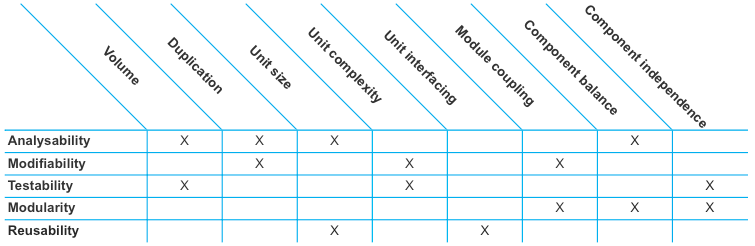
\includegraphics[width=0.8\linewidth]{figs/mmodel.png}
  \caption{Maintainability model}
  \label{fig:mmodel}
\end{figure}


%%% Local Variables:
%%% mode: latex
%%% TeX-master: "IWSM-Mensura-2016"
%%% End:
